\documentclass[a4paper, 10pt]{article}
\usepackage{graphicx} % Required for inserting images
\usepackage[utf8]{inputenc}
\usepackage[german]{babel}
\usepackage{geometry}
\usepackage{fancyhdr}
\usepackage{titlesec}
\usepackage{xcolor}
\usepackage{enumitem}
\usepackage{lipsum}
\usepackage{tcolorbox}
\usepackage{amsmath} % Für mathematische Formeln (optional)
\usepackage{xcolor}  % Für Farbdefinitionen
\usepackage{soul}    % Für Textmarkierung
%Seitenlayout
\geometry{top=2.5cm, left=2cm, right=2cm}

%Kopf- und Fußzeile
\pagestyle{fancy}
\fancyhf{}
\fancyhead[L]{\textbf{Mikroökonomie 2024/25}}
\fancyhead[R]{\textbf{Lena Thuy Trang Vo}}
\fancyfoot[C]{\thepage}

%Farben 
\definecolor{lightpink}{rgb}{1.0, 0.75, 0.8}
\definecolor{darkpink}{rgb}{1.0, 0.5, 0.7}

% Titel-Formatierung
\titleformat{\section}{\large\color{darkpink}\bfseries}{}{0em}{}[\titlerule]
\titleformat{\subsection}{\color{darkpink}\bfseries}{}{0em}{}

% Definition-Box
\newtcolorbox{definitionbox}{
  colback=lightpink, % Hintergrundfarbe
  colframe=darkpink, % Rahmenfarbe
  fonttitle=\bfseries,
  title=Definition,
  boxrule=0.8mm, % Dicke des Rahmens
  width=\textwidth, % Breite der Box
  before=\vspace{0.5cm}, % Abstand vor der Box
  after=\vspace{0.5cm}, % Abstand nach der Box
  sharp corners=south % Scharfe Ecken unten
}

\definecolor{lightpink}{rgb}{1.0, 0.75, 0.8}
% Befehl für das Hervorheben
\sethlcolor{lightpink} % Setze die Highlight-Farbe

\begin{document}

\begin{titlepage}
    \centering
    \vspace*{3cm}
    {\Huge \textbf{Mikroökonomie}}\\[1.5cm]
    {\large \textit{Lena Thuy Trang Vo}}\\[0.5cm]
    {\large \textit{Wintersemester 2024/25}}\\[2cm]

    \vfill
\end{titlepage}

\tableofcontents
\newpage

\section{Einführung}
Mikroökonomik ist ein Teilbereich der Wirtschaftswissenschaften, der sich mit dem Verhalten von Individuen und Unternehmen sowie deren Interaktionen auf Märkten beschäftigt. Im Mittelpunkt stehen die Entscheidungsprozesse von Haushalten und Unternehmen, die Preisbildung auf Märkten sowie die Allokation knapper Ressourcen. Mikroökonomik analysiert, wie diese Akteure ihre Entscheidungen unter Berücksichtigung von Knappheit und Anreizen treffen, und untersucht die Auswirkungen dieser Entscheidungen auf Angebot und Nachfrage, Marktgleichgewichte und die Verteilung von Ressourcen.


\section{Die Nachfrageseite}
\subsection{Motivation}

\textbf{Aggregierte Nachfrage}
\begin{itemize}
    \item repräsentiert die Gesamtnachfrage aller Konsumenten nach Gütern und Dienstleistungen in einer Volkswirtschaft bei verschiedenen Preisniveaus
    \item zusammen mit dem Angebot bestimmt sie die Preise und den Konsum auf Märkten
    \item gibt Aufschluss darüber, wer wie viel konsumiert und wie es um die Konsumentenwohlfahrt steht
\end{itemize}

\begin{definitionbox}
    Die Konsumentenwohlfahrt ist ein Maß für den Nutzen oder die Zufriedenheit, die Konsumenten aus dem Konsum von Gütern und Dienstleistungen ziehen. Sie wird oft durch die Konsumentenrente dargestellt, welche die Differenz zwischen dem maximalen Preis, den Konsumenten bereit sind zu zahlen, und dem tatsächlich gezahlten Preis darstellt.
\end{definitionbox}

\textbf{Individuelle Nachfrage}
\begin{itemize}
    \item bezieht sich auf das Kaufverhalten/Entscheidungdverhalten eines einzelnen Konsumenten
    \item hängt ab von:
    \begin{itemize}
    \item \hl{Präferenzen:} spiegeln individuelle Bedürfnisse und Wünsche wider, die bestimmen, welche Produkte bevorzugt werden
    \item \hl{Budget:} das verfügbare Einkommen des Konsumenten ist begrenzt, welche Güter und Dienstleistungen er sich leisten kann
    \item \hl{rationales Verhalten:} Konsumenten handeln nuzuenmaximierend, indem sie versuchen, das beste Verhältnis zwischen Preis und Nutzen zu erzielen
\end{itemize}
\end{itemize}


\subsection{Budget}
\textbf{Der Zweigüterfall}\\
Im Zweigüterfall betrachten wie die Konsumentscheidungen eines Individuums \textit{zwischen zwei Gütern}, die \textit{ohne Beschränkung der Allgemeinheit} als Waren, Dienstleistungen oder andere Dinge wie frische Luft angesehen werden können.\\
Ein \textit{\hl{Güterbündel}} wird als $x \equiv (x_1, x_2)$ dargestellt, wobei $x_i \geq 0$ die \textit{\hl{konsumierte Menge}} des jeweiligen Guts darstellt.\\
Die dazugehörigen \textit{\hl{Preise}} $p_i$ pro Einheit sind für Konsumenten gegeben und einheitlich. \\
Das \textit{\hl{verfügbare Budget}} des Konsumenten ist $m$.\\[4mm]
\textbf{Budgetbeschränkung: Was kann man sich leisten?}\\
Die \hl{Budgetmenge} enthält alle Güterbündel, die bei den aktuellen Preisen erschwinglich sind \\
\begin{equation}
    x'p = p_1 x_1 + p_2 x_2 \leq m
\end{equation}\\
Sie wird durch die \hl{Budgetgerade} abgegrenzt, also die Menge aller Güterbündel, die das Budget vollkommen erschöpfen
\begin{equation}
    x_2 = \frac{m}{p_2} - \frac{p_1}{p_2}x_1
\end{equation}
Die Steigung zeigt an, mit welcher Rate die beiden Güter auf der Budgetgerade füreinander subsstituiert werden können, also die \hl{Opportunitätskosten}.

\begin{definitionbox}
    Opportunitätskosten sind allgemein die ökonomischen Kosten einer Entscheidung, also der Wert der nächstbesten ungenutzten Alternative. Im Kontext der
Budgetgeraden entsprechen diese der Steigung:
\begin{equation}
    \frac{dx_2}{dx_1} = - \frac{p_1}{p_2}
\end{equation}
\end{definitionbox}

\subsection{Präferenzen und Nutzen}
\textbf{Präferenzen: Was möchte man haben?}\\
In der Volkswirtschaftslehre modellieren wir die Bedürfnisse und Wünsche der Menschen anhand von \hl{Präferenzen}.\\
Nehmen wir zwei Güterbündel:
\begin{itemize}
    \item $x=(x_1,x_2)$
    \item $y = (y_1, y_2)$
\end{itemize}
In diesem Fall steht $x_1$ und $y_1$ für die Menge eines Iphone 15 und $x_2, y_2$ für die Menge eines Samsung S24.
\\[3mm]
\textbf{Präferenzrelationen}
\begin{enumerate}
    \item \hl{Strikte Präferenz $\succ$:} 
    \begin{itemize}
        \item zeigt, dass ein Konsument, ein Güterbündel dem anderen strikt vorzieht
        \item  Beispiel:\\
    $(1,0) \succ (0,1)$ Iphone 15 wird bevorzugt
    \end{itemize}
    
    \item \hl{Indifferenz $\sim$:}
    \begin{itemize}
        \item bedeutet, dass der Konsument zwischen den beiden Güterbündeln keinen Unterschied in der Präferenz sieht
        \item Beispiel:\\
        $(1,0) \sim (0,2)$ \\ Sie sind indifferent, ob sie nur das Iphone 15 oder zwei Samsung S24 erhalten. Beide Bündel sind für sie gleichwertig.
    \end{itemize}

    \item \hl{Schwache Präferenz $\succeq$}
    \begin{itemize}
        \item bedeuetet, dass der Konsument ein Güterbündel mindestens genau so gut findet wie ein anderes, aber er findet es nicht unbedingt besser
        \item Beispiel:\\
        $(1,0) \succeq (0,1)$\\
        Sie haben eine schwache Präferenz für das iPhone 15 über das Samsung S24. Sie bevorzugen das iPhone 15, aber vielleicht nicht strikt.
    \end{itemize}
\end{enumerate}
\noindent \textbf{Vernünftige Präferenzen}\\
In der Volkswirtschaftslehre gehen wir oft davon aus, dass die Präferenzen von Konsumenten bestimmte Eigenschaften erfüllen, um die Modellierung und das Verständnis des Konsumverhaltens zu erleichtern. Solche \hl{„wohlverhaltenen“ Präferenzen} sind nützlich, um verlässliche Aussagen über das Verhalten der Konsumenten zu treffen.
\begin{enumerate}
    \item \hl{vollständig}\\
    $x \succeq y \, \lor \, y \succeq x \quad \forall x, y$
    \item \hl{reflexiv}\\
    $x \succeq x \quad \forall x$
    \item \hl{transitiv}\\
    $x \succeq y \, \land \, y \succeq z \implies x \succeq z \quad \forall x, y, z$
    \item \hl{monoton (keine Sättigung)}\\
    $x_i \geq y_i \, \forall i \implies x \succeq y$
    \item \hl{stetig}
\end{enumerate}

\noindent \textbf{Die Nutzenfunktion}
\begin{itemize}
    \item dient dazu, die Präferenzen von Konsumenten mathematisch abzubilden
    \item ordnet jedem Güterbündel einen numerischen Wert zu, der den Nutzen oder die Zufriedenheit des Konsumenten mit diesem Bündel widerspiegelz
    \item werden zumeist als $u(x) = u (x_1, x_2)$ notiert
\end{itemize}

\noindent \textbf{Kardinaler vs. Ordinaler Nutzen}\\
Der \textbf{kardinale Nutzen} war in den Anfängen der Ökonomie als \hl{messbar} und \hl{absolut} angesehen, was bedeutete, dass man glaubte, den Nutzen in \hl{konkreten Einheiten quantifizieren} zu können. Im Gegensatz dazu betrachtet der \textbf{ordinale Nutzen} nur die \hl{Rangordnung von Präferenzen}, \hl{ohne dass die absoluten Unterschiede} im Nutzenwert eine Bedeutung haben. Dies erlaubt es, monotone Transformationen auf die Nutzenfunktion anzuwenden, wobei die zugrunde liegenden Präferenzen unverändert bleiben.\\

\noindent\textbf{Beispiele für Nutzenfunktionen}\\
\hl{Perfekte Substitute}
\begin{equation}
    u(x) = x_1 + x_2
\end{equation}
Diese Funktion impliziert, dass die Güter vollständig austauschbar sind und der Konsument indifferent ist zwischen den Gütern, solange die Gesamtmenge gleich bleibt.\\

\noindent\hl{Perfekte Komplemente}
\begin{equation}
    u(x) = \min\{x_1, x_2\}
\end{equation}
Diese Funktion beschreibt Güter, die nur in festen Verhältnissen konsumiert werden können, wie etwa linke und rechte Schuhe.\\

\noindent\hl{Cobb-Douglas}
\begin{equation}
    u(x) = x_1^{\alpha} x_2^{1-\alpha}
\end{equation}
Diese Funktion modelliert Präferenzen mit konstanter Elastizität der Substitution und ist weit verbreitet in der Ökonomie.\\

\noindent \hl{Quasilineare Präferenzen}
\begin{equation}
    u(x) = v(x_1) + x_2, \quad \text{mit} \quad v'(x_1) > 0, \, v''(x_1) < 0
\end{equation}
Diese Funktion beschreibt Präferenzen, bei denen der Grenznutzen eines Gutes konstant bleibt und nicht vom Konsum des anderen Gutes abhängt.\\

\noindent\textbf{Grenznutzen}\\
Um das beste Güterbündel ohne Budgetrestriktion zu finden, betrachten wir den Grenznutzen eines Gutes.\\
Der Grenznutzen beschreibt den \hl{zusätzlichen Nutzen}, den ein Konsument durch den Konsum einer weiteren Einheit eines Gutes erhält.\\[2.5mm]
\begin{definitionbox}
    Mathematisch ist der Grenznutzen die erste Ableitung der Nutzenfunktion $u(x)$ nach der Menge des Gutes $x$, also
    \begin{equation}
        \frac{\partial u(x)}{\partial x_i} \equiv MU_i. 
    \end{equation}
\end{definitionbox}\\
Wenn wir uns entscheiden müssen, ob wir mehr oder weniger von einem Gut konsumieren wollen, vergleichen wir den Grenznutzen mit dem Preis (in Nutzen gemessen).
\begin{itemize}
    \item Wenn der Grenznutzen der nächsten Einheit größer als der Preis ist, lohnt es sich, mehr zu konsumieren. Dies bedeutet, dass der zusätzliche Nutzen, den wir aus einer weiteren Einheit ziehen, die Kosten übersteigt.
    \item Ist der Grenznutzen niederiger als der Preis, sollten wir den Konsum reduzieren, da die zusätzlichen Kosten den Nutzen übersteigen.
    \item typischerweise fällt der Grenznutzen eines Gutes, wenn man mehr konsumiert
    \item mit mehreren Gütern ist es komplizierter, aber der Grenznutzen wird dennoch eine zentrale Rolle spielen
\end{itemize}
\begin{figure}
    \centering
    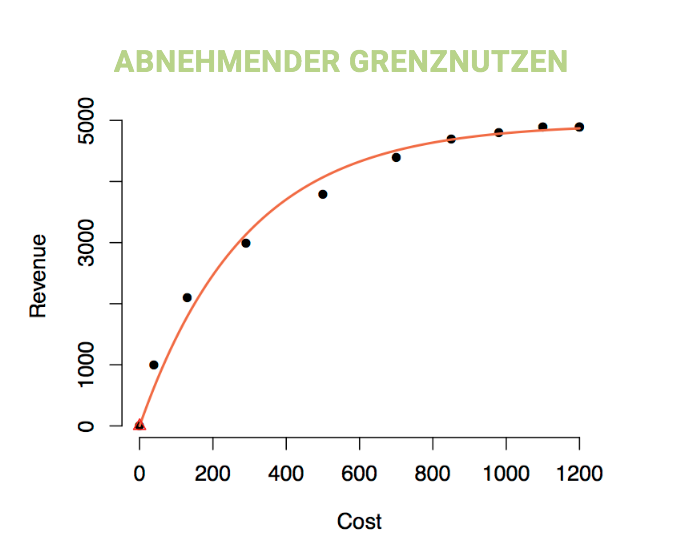
\includegraphics[width=0.4\linewidth]{/Users/lenavo/Desktop/3.Semester/Mikroökonomie/img/grenznutzen.png}
    \caption{Grenznutzen}
    \label{fig:enter-label}
\end{figure}
\textbf{Indifferenzkurven}\\
Indifferenzkurven sind ein zentrales Konzept in der Mikroökonomie, das verwendet wird, um die \hl{Präferenzen eines Konsumenten zwischen verschiedenen Güterbündeln} darzustellen. Sie zeigen alle Kombinationen von zwei Gütern, bei denen der Konsument den gleichen Nutzen erfährt und somit \hl{indifferent} ist.

\begin{itemize}
    \item Sie sind Mengenscharen aller Güterbündel, die den gleichen Nutzenwert erzeugen; also solche, zwischen denen
ein:e Konsument:in indifferent ist
\begin{equation}
    \{ x \mid u(x) = \bar{u} \}
\end{equation}
    \item Ihre Form zeigt uns, wie gerne wir substitutieren, also freiwillig von einem Gut weniger und von anderen
mehr konsumieren würden
\end{itemize}
Um das beste Güterbündel – also die Nachfrage – zu finden, wollen wir die höchste Indifferenzkurve finden, auf der
mind. ein Güterbündel in der Budgetmenge liegt.
\begin{itemize}
    \item Es wird also ein Tangenzialpunkt gesucht: Im Optimum ist die Steigung der Indifferenzkurve genauso groß wie
die Steigung der Budgetgeraden!
\end{itemize}
Die \hl{Steigung der Indifferenzkurve} wird als \hl{Grenzrate der Substitution} bezeichnet (Marginal Rate of
Substitution)
\begin{itemize}
    \item Für ein beliebiges Nutzenniveau $k$ und eine Nutzenfunktion für zwei Güter $u(x_1, x_2)$: 
\end{itemize}
\begin{equation}
    du(x_1, x_2) = dk = 0 = \frac{\partial u}{\partial x_1} dx_1 + \frac{\partial u}{\partial x_2} dx_2 \Leftrightarrow
\end{equation}

\begin{equation}
    \frac{dx_2}{dx_1} =\underbrace{ - \frac{\frac{\partial u}{\partial x_1}}{\frac{\partial u}{\partial x_2}}}_{\text{Grenzrate der Substitution}} \equiv  - \frac{MU_1}{MU_2} \equiv MRS_{1,2}
\end{equation}
\textbf{Eigenschaften der MRS}
\begin{itemize}
    \item ist bei differenzierbaren Nutzenfunktionen \hl{negativ}
    \item wenn man von einem Gut mehr konsumiert, kann man \hl{ohne Nutzenverlust} weniger von einem anderen konsumieren
    \item sie gibt den \hl{''Wechselkurs''} an, zu der Konsument:innen bereit sind, Güter füreinander auszutauschen
    \item bei \hl{schwach konvexen Präferenzen} fällt die MRS nicht, bei \hl{strikt konvexen Präferenzen} steigt sie
    \item d.h. $|MRS|$ nimmt typischerweise schwach ab
    \item man muss also immer mehr von einem Gut aufgeben, um den Nutzen durch Konsum des anderen Gutes konstant zu halten
\end{itemize}
\subsection{Individuelle Nachfrage}
\begin{itemize}
    \item beschäftigt sich nur mit Konsument
\end{itemize}
\textbf{Der Lagrange-Ansatz}
\begin{itemize}
    \item Problem: Güterbündel finden, mit dem wir den \hl{Nutzen maximieren} (unter Einhaltunf der Budgetbedingung):
            \[
            \max_{x} \quad u(x) \quad \text{u.d.N.} \quad x'p \leq m
            \]

    \item wir verwenden die \hl{Lagrange-Methode} mit Multiplikator $\lambda$:
            \[
                \max_{x, \lambda} \quad \mathcal{L} = u(x) + \lambda(m - x'p)
            \]
            \begin{itemize}
                \item Zielfunktion + Nebenbedingung 
                \item wenig Budget $\rightarrow$ Lambda sehr groß, viel Budget $\rightarrow$ Lambda sehr klein
            \end{itemize}


    \item \hl{notwendigen Bedingung erster Ordnung} finden $\rightarrow$ nach $x_i$ ableiten
    \item die notwendigen Bedingungen erster Ordnung geben uns ein \hl{Gleichungssystem}, das wir für $x^*$, $\lambda^*$ lösen können
                \[
\frac{\partial u(\cdot)}{\partial x_i} \bigg|_{x^*} = MU_i \bigg|_{x^*} = \lambda^* p_i \quad \forall i
\]
\[
m = x^{*'} p
\]
    \item alle Optimalen Lösungen mit einem * kennzeichnen
\end{itemize}
\textbf{Optimale Nachfrage}
\begin{itemize}
    \item dividieren wir die Bedingungen erster Ordnung für zwei Güter $i$ und $j$ durcheinander und multiplizieren mit (-1), so erhalten wir die \hl{Steigung der Budgetgeraden}
    \newpage
    \begin{figure}[h]
        \centering
        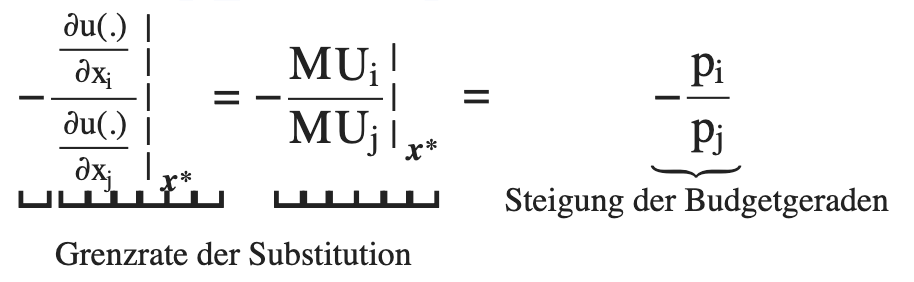
\includegraphics[width=0.5\linewidth]{/Users/lenavo/Desktop/3.Semester/Mikroökonomie/img/optnachf.png}
        \caption{Steigung der Budgetgeraden}
        \label{fig:enter-label}
    \end{figure}

    \item linke Seite des Ausrucks ist die \textbf{Grenzrate der Substitution}, welche das \hl{Austauschverhältnis} zwischen den Gütern beschreibt, bei dem der Konsument auf einem \hl{konstanten Nutzenniveau} bleibt
    \item rechte Seite: Verhältnis der Preise, also \textbf{Steigung der Budgetgeraden} 
\end{itemize}
\textbf{Beispiel:}
Wenn für ein suboptimales Güterbündel gilt:
\[
    MRS(x_1',x_2') > \frac{p_1}{p_2}
\]
\begin{itemize}
    \item dann ist der relative Grenznutzen von Gut 1 \textbf{höher als das Preisverhältnis} 
    \item Konsument würde in dem Fall \textbf{mehr von Gut 1} konsumieren wollen und weniger von Gut 2, da er mit dem aktuellen Konsumplan nicht seinen maximalen Nutzen erreicht
    \item der \hl{Langrage-Multiplikator} $\mathcal{L}$, auch als \textbf{Schattenpreis} des Einkommens bezeichnet, gibt den \hl{zusätzlichen Nutzen} an, den ein Konsument durch eine \hl{marginale Erhöhung} seines Einkommens erzielen würde 
\end{itemize}
\textbf{Beispiel: Cobb-Douglas}
\begin{itemize}
    \item Nehmen wir Cobb-Douglas Präferenzen an, also:
    \[
        u(x_1,x_2) = x_1^\alpha x_2^{1- \alpha}   \qquad \text{mit} \quad a \in (0,1)
    \]

    \item um die optimale Nachfrage nach den Gütern $x_1$ und $x_2$ zu bestimmen, kann man die \hl{Langrage-Methode} verwenden oder direkt die bekannten \hl{Nachfragefunktionen ableiten}
\end{itemize}
\hl{Schritt 1: Lagrange-Funktion aufstellen}
\[
    \mathcal{L}(x_1,x_2) = x_1^\alpha \cdot x_2^{1- \alpha} + \lambda (m - p_1 x_1 - p_2 x_2)
\]  
Erinnerung: $\lambda$ stellt Schattenpreis dar\\[2mm]
\hl{Schritt 2: Erste Ordnung Bedingungen (FOCS)}\\[1.5mm]
Wir leiten nach $x_1$, $x_2$ und $\lambda$ ab und setzen die Ableitungen gleich 0 \\[1.5mm]
\textbf{Ableitung nach $x_1$:}
\[
    \frac{\delta \mathcal{L}}{\delta x_1} = \alpha x_1^{\alpha -1}x_2^{1- \alpha} - \lambda p_1 = 0
\]

\noindent\textbf{Ableitung nach $x_2$:}
\[
    \frac{\delta \mathcal{L}}{\delta x_2} = (1 - \alpha) x_1^\alpha x_2^{- \alpha} - \lambda p_2 = 0
\]
\textbf{Ableitung nach $\lambda$:}
\[
    \frac{\delta \mathcal{L}}{\delta \lambda} = m - p_1 x_1 - p_2 x_2 = 0
\]

\noindent\hl{Schritt 3: Verhältnis der Grenznutzen}\\[1.5mm]
Um die optimale Nachfrage zu bestimmen, dividieren wir die erste Bedinung durch die zweite
\[
    \frac{ax_1^{\alpha - 1} x_2^{\alpha -1}}{(1 - \alpha) x_1^\alpha x_2^{- \alpha}} = \frac{\lambda p_1}{\lambda p_2}
\] 

\[
    \frac{\alpha}{(1 - \alpha)} \cdot \frac{x_2}{x_1} = \frac{p_1}{p_2}
\]
Nach Umstellen:
\[
    x_2^* = \frac{(1 - \alpha)}{\alpha} \cdot \frac{p_1}{p_2} \cdot x_1^*
\]
\hl{Schritt 4: Einsetzen in die Budgetgleichung}\\[1.5mm]
Nun setzen wir diese Beziehung in die Budgetbeschränkung ein.
\[
    m = p_1 x_1^* + p_2 x_2^*
\]
Setzen wir den Ausdruck für $x_2^*$ in diese Gleichung ein:
\[
    m = p_1 x_1^* + p_2 (\frac{(1- \alpha)}\alpha{} \cdot \frac{p_1}{p_2} x_1^*)
\]
\begin{itemize}
    \item mit Cobb-Douglas Präferenzen gibt man einen konstanten Teil $\alpha$ für Gut 1 und den Rest für Gut 2 aus
\end{itemize}
\subsection{Eigenschaften der individuellen Nachfrage}
\subsubsection{Einkommens-Expansionspfade, Engel-Kurven und Gütertypen}
\textbf{Einkommens-Expansionspfad}
\begin{itemize}
    \item zeigt, wie sich die \hl{optimale Konsummenge} zweier Güter verändert, wenn das \hl{Einkommen zunimmt}, während die \hl{Preise der Güter konstant} bleiben
    \item \textbf{normale Güter:} Einkommens-Expansionspfad hat eine \hl{positive Steigung} $\rightarrow$ bedeutet, dass mit steigendem Einkommen mehr von beiden Gütern konsumiert wird
    \item \textbf{inferiore Güter:} Einkommens-Expansionspfad kann \hl{"gewunden"} sein, d.h. nach einer \textbf{anfänglichen Steigung} könnte er \textbf{abfallen}
    \begin{itemize}
        \item ab einem \textbf{bestimmten Einkommensniveau} wird \hl{weniger von dem inferioren Gut} konsumiert, da der Konsument auf \hl{höherwertige Alternativen} umsteigt
    \end{itemize}
\end{itemize}

\noindent\textbf{Engel-Kurve}
\begin{itemize}
    \item stellt Beziehung zwischen dem Einkommen und der nachgefragten Menge eines Gutes dar
    \item hat für \textbf{normale Güter} eine \hl{positive Steigung} $\rightarrow$ Nachfrage nach Gut nimmt mit steigendem Einkommen zu
    \item \textbf{inferiore Güter:} Engel-Kurve hat eine \hl{negative Steigung ab einem bestimmten Einkommensniveau} $\rightarrow$ Nachfrage nach dem Gut nimmt ab, wenn das Einkommen weiter steigt
    \begin{itemize}
        \item tritt häufig bei \textbf{niedrigpreisigen oder qualitativ minderwertigen} Produkten auf, die durch höherwertige Alternativen ersetzt werden
    \end{itemize}
\end{itemize}

\begin{definitionbox}
    \textbf{Inferiores Gut:} Ein Gut, dessen Nachfrage bei steigendem Einkommen sinkt (z.B Instantnudeln, gebrauchte Kleidung)\\[2mm]
    \textbf{Notwendiges Gut:} Ein Gut, dessen Nachfrage mit steigendem Einkommen zunimmt, aber langsamer als das Einkommen selbst (z.B. Grundnahrungsmittel)\\[2mm]
    \textbf{Luxusgut:} Ein Gut, dessen Nachfrage schneller als das Einkommen steigt (z.B. teure Autos oder Schmuck)
\end{definitionbox}
\newpage
\begin{figure}[h]
    \centering
    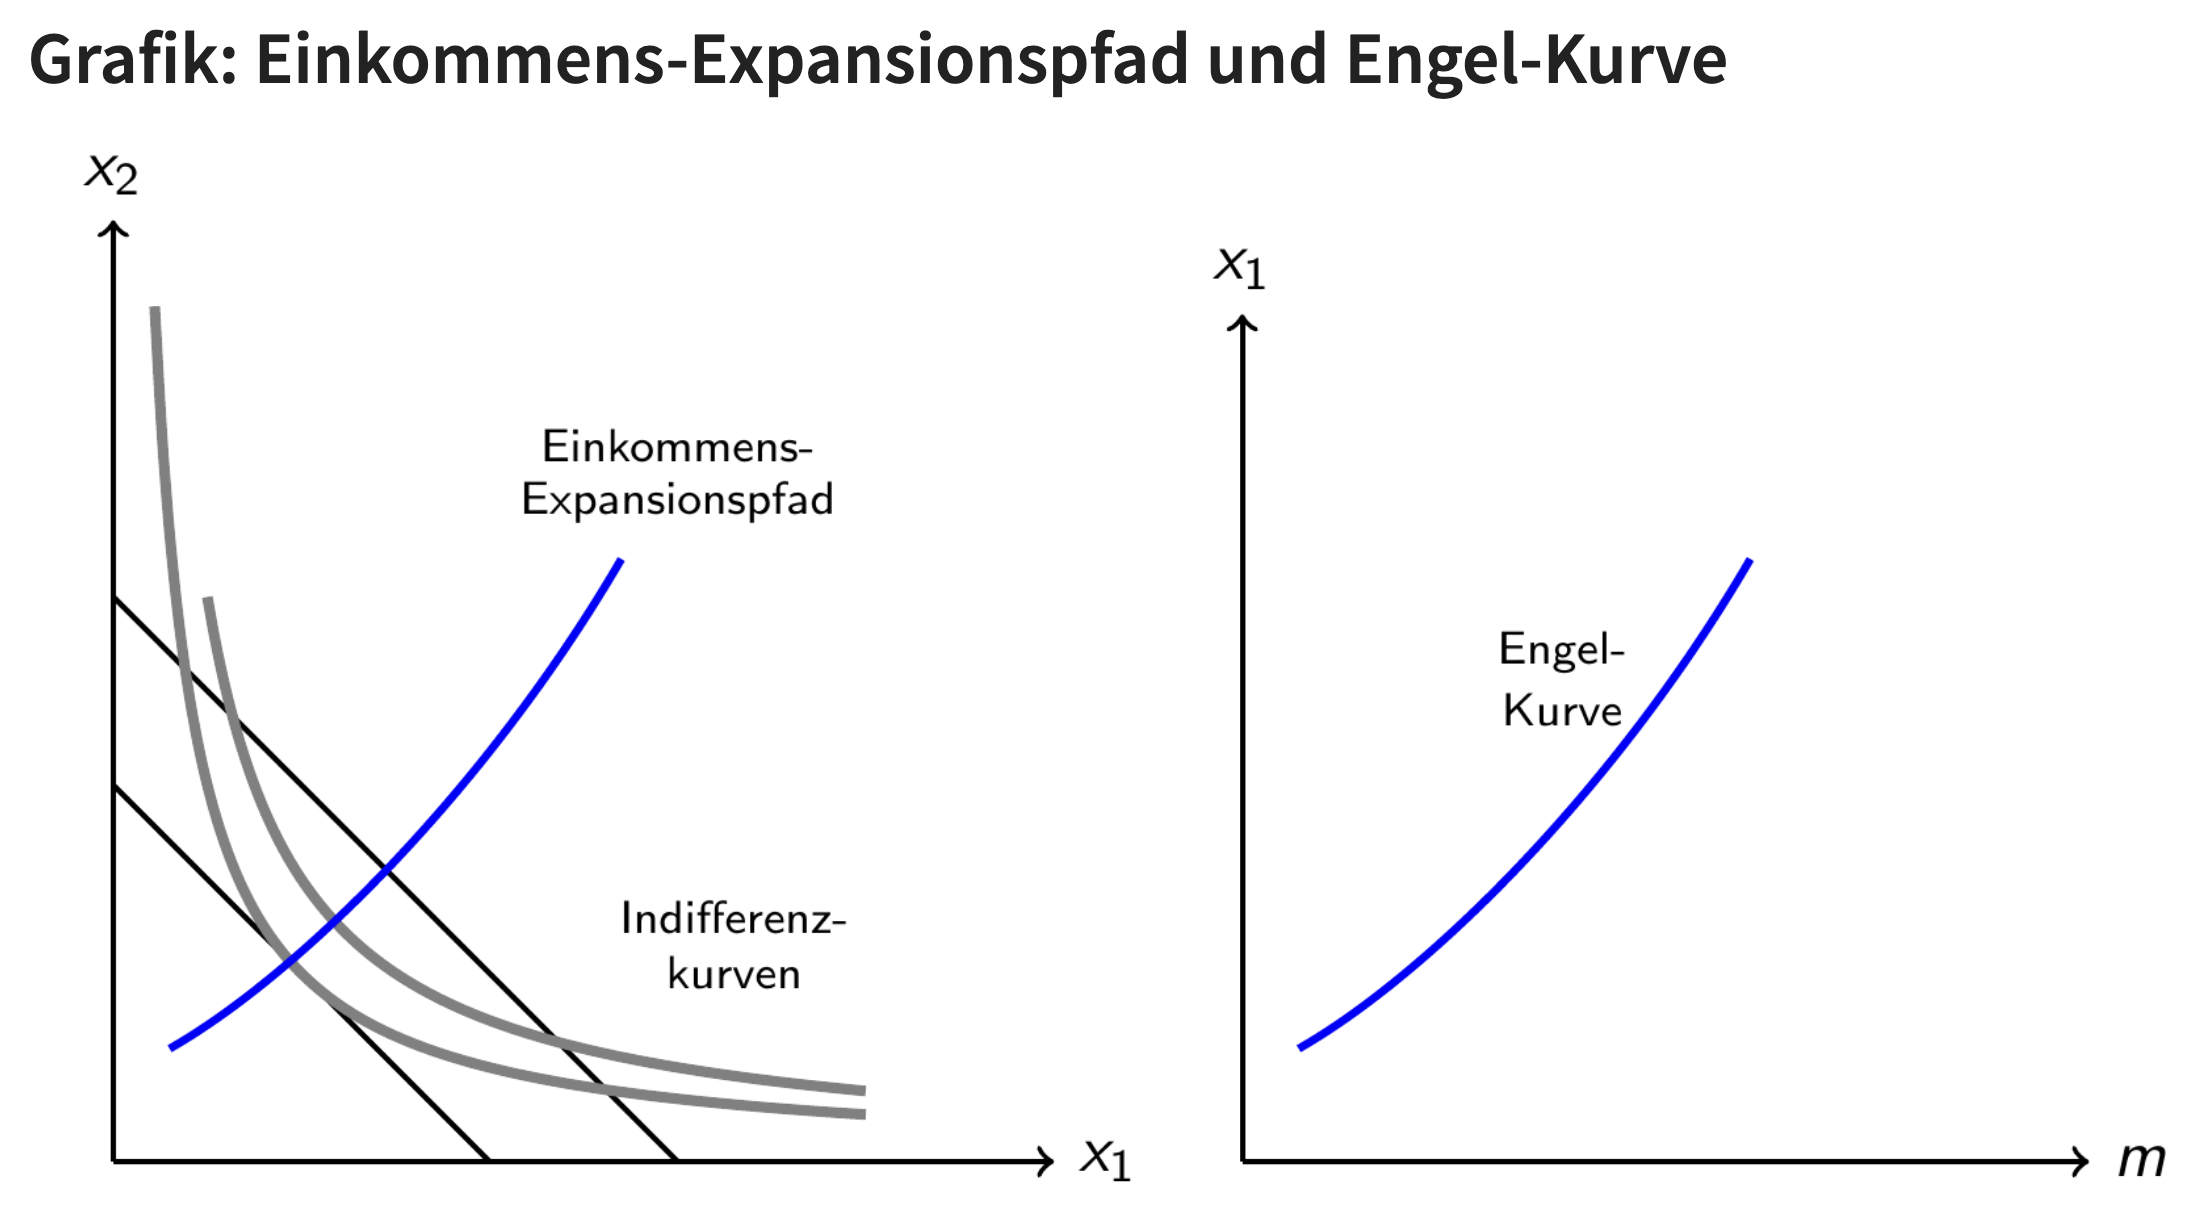
\includegraphics[width=0.5\linewidth]{/Users/lenavo/Desktop/3.Semester/Mikroökonomie/img/engelskurve.png}
    \caption{}
    \label{fig:enter-label}
\end{figure}
\subsubsection{Die Slutsky-Zerlegung}
\begin{itemize}
    \item teilt die Auswirkungen einer Preisänderung auf die Nachfrage nach einem Gut in zwei Komponenten auf
    \item Giffen-Gut $\rightarrow$ optimale Nachfrage nach einem Gut geht zurück, wenn sein Preis fällt
    \begin{itemize}
        \item Einkommenseffekt ist so stark, dass er den Substitutionseffekt überkompensiert
    \end{itemize}
\end{itemize}
Preissteigerung hat immer zwei Effekte:
\begin{enumerate}
    \item \textbf{Substitutionseffekt}
    \begin{itemize}
        \item beschreibt, wie sich die Nachfrage ändert, wenn der \hl{relative Preis eines Gutes steigt}, während das \hl{reale Einkommen konstant bleibt}
        \item Substitutionseffekt: die Nachfrageänderung aufgrund der Änderung des Tauschverhältnisses
    \end{itemize}


    \item \textbf{Einkommenseffekt}
    \begin{itemize}
        \item Nachfrageänderung aufgrund \hl{gestiegener Kaufkraft}
    \end{itemize}
\end{enumerate}
\begin{figure}[h]
    \centering
    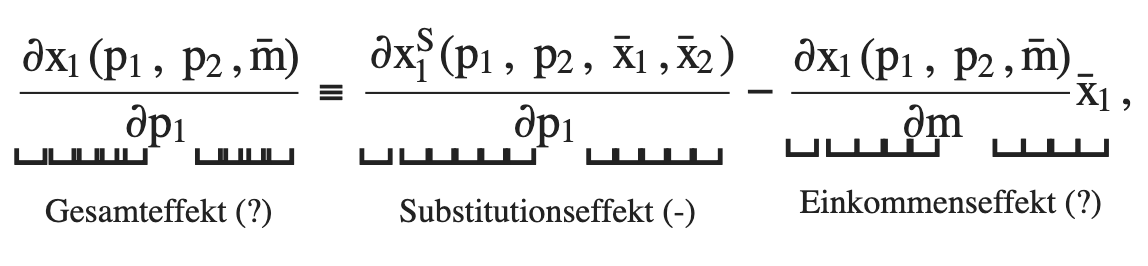
\includegraphics[width=0.6\linewidth]{/Users/lenavo/Desktop/3.Semester/Mikroökonomie/img/slutzky.png}
    \caption{Slutzky-Identität}
    \label{fig:enter-label}
\end{figure}

\end{document}
